\documentclass[11pt]{article}

\usepackage[table, svgnames, dvipsnames]{xcolor}
\usepackage[final]{acl}
% Download the ACL style files from the link below.
% You need the `acl.sty' and `acl_natbib.bst' files, keep these in the same
% directory as your TeX file.
% https://github.com/acl-org/acl-style-files/tree/master/latex
\usepackage{times}
\usepackage{latexsym}
\usepackage[T1]{fontenc}
\usepackage[utf8]{inputenc}
\usepackage{microtype}
%\usepackage{inconsolata}
\usepackage{hyperref}
\usepackage{graphicx}
\usepackage{todonotes}
\usepackage{amsmath}
\usepackage{algorithm}
\usepackage{subcaption}
\usepackage{algpseudocode}

%\bibliographystyle{acl}


\makeatletter
\def\endthebibliography{%
  \def\@noitemerr{\@latex@warning{Empty `thebibliography' environment}}%
  %\endlist
}
\makeatother


\title{Affective Speech Synthesis - A Comparison}

\author{Hannes Bachmann\\
  4847472\\
  INF-BAS2 \\
  \texttt{\small hannes.bachmann@mailbox.tu-dresden.de}
  \\ \And
  Julia Rennert \\
  4924490\\
  INF-VERT2 \\
  \texttt{\small julia.rennert@tu-dresden.de}
  }
  
\definecolor{ashgrey}{rgb}{0.7, 0.75, 0.71}
\definecolor{gainsboro}{rgb}{0.86, 0.86, 0.86}
\definecolor{mintgreen}{rgb}{0.6, 1.0, 0.6}


\begin{document}
\maketitle
\begin{abstract}
Speech synthesis has become a common tool over the past few decades. This opens up the questions whether the synthesized speech can be given a more life-like sounding, namely emotionalism, a problem that is accumulated in the field of affective speech synthesis. \\
In our project, we compare modern technologies in emotion recognition and text-to-speech with common methodologies of acoustics, using both to extract a sentence's prevalent emotion and transform it into emotional speech. We also create a benchmark to evaluate our methods in contrast to the common solutions.
\end{abstract}

\section{Introduction}
Speech synthesis has evolved from a difficult problem to a common tool over the past few decades.
It started with simulating mouth movements, then moved on to rule-based, concatenative and
statistical synthesis, and then to using deep learning. Today, synthesized speech is used in a
variety of applications, such as voice assistants and video dubbing.
While general speech synthesis has already made good progress, work is still being done on
how to give language a specific characteristic. To define this problem, the information content of
the spoken word is divided into three areas. First, there is the content of the text, more or less
a transcript of what is being said. Then there is the emotion that the speaker conveys through
his voice. And thirdly, there is the identity of the speaker himself, which is also characterized by
his voice. Affective Speech Synthesis, also called emotional text-to-speech (ETTS), refers to the change in emotion while the other two areas remain the static.

The most successful current approaches are based on deep learning\cite{triantafyllopoulos_overview_2023, cho_multi-speaker_2021, diatlova_emospeech_2023}. This warrants the question, whether a more traditional acoustic-based approach can still compare to some extend. For this purpose, we tried to apply two competing approaches to the problem of ETTS, one up to the current deep learning methods, and one a deep dive in the waters of acoustics. Our second requirement is to create a general benchmark as the evaluation of ETTS is still not standardized.

In Section \ref{related_work}, we will discuss the basics of (affective) speech synthesis and the current research. Our own methodologies will be introduced in Section \ref{methodology}. Then we evaluate the methods in  Section \ref{evaluation} by comparing the outcomes to each other and two approaches of previous research, where one of them is a current deep learning approach and one a more traditional statistical method. We discuss the outcome in Section \ref{discussion} and summarize our findings in Section \ref{conclusion}.

\begin{table}[h]

\vspace{5px}
{
%\hspace{-15px}
\begin{tabular}{|l|l|l|}
\hline
\rowcolor{gainsboro}&our method&external method\\
\hline
\cellcolor{gainsboro}deep learning&Approach 1&EmoSpeech\\
\hline
\cellcolor{gainsboro}acoustic&Approach 2&Affect Editor\\
\hline

\end{tabular}

}
\caption{Goal of the evaluation}
\end{table}


\section{Related Work}
\label{related_work}
\subsection{Groundwork}
To understand the ongoings in the research area of ETTS, let us first take a short look at regular speech synthesis. The beginning of speech synthesis lies in articulatory synthesis where the scientists tried to remodel the movements of the oral articulators. It was followed by the format synthesis where rule-based changes to amplitudes and frequencies of an oscillating source were made. Unfortunately, it turned out to be complicated to find the needed rules. This approach was followed by the concatenative speech synthesis where prerecorded phonemes, syllables or words were used to construct the speech. As this kind of synthesis needs a lot of prerecorded data and the output has lapses in continuity, it was abandoned for statistical parametric speech synthesis. This kind of synthesis consists of three stages, text analysis to find the correct pronunciation of the given words, the prediction of the speech parameters by using an acoustic model and the vocoding, the construction of the waveform. These stages could include machine learning, oftentimes hidden Markov models. With the upcoming of deep learning, this system was complemented by deep neuronal networks \cite{triantafyllopoulos_overview_2023,shen_natural_2018}.

Affective speech synthesis mostly uses the progress made in regular speech synthesis by utilizing its methods. The first ETTS algorithms were rule-based like in format synthesis. A very successful example for this type of synthesis is the Affect Editor of \cite{cahn_generation_2000}. Just as in regular speech synthesis, this method was followed by a concatenative approach, as for example used by \cite{pierre-yves_production_2003} to model emotional babbling. Finally, the ETTS reached a data-driven stage as well.
Nowadays emotional speech synthesis has two predominating methods. Text-to-emotional-features synthesis tries to extract the emotional utterances directly from the text, while emotional voice conversion goes the step over the regular speech synthesis and then applies the emotion to the pre-created speech. Due to the higher progress in normal speech synthesis research, the second approach is used more frequently.

Another distinguisher is made by the type of data that is available for the training. If there is a corpus of data from the same speaker and the same sentence with different underlying emotion, one speaks of parallel data. This kind of data is easy to learn from since you do not have to distinguish between different speakers or different situations, but hard to get, as it mostly requires talented vocal artists to record it. Therefore, an active part of research is how to cope with non-parallel data, that is from different speakers or with different textual content.

\begin{figure}[h]
 \centering
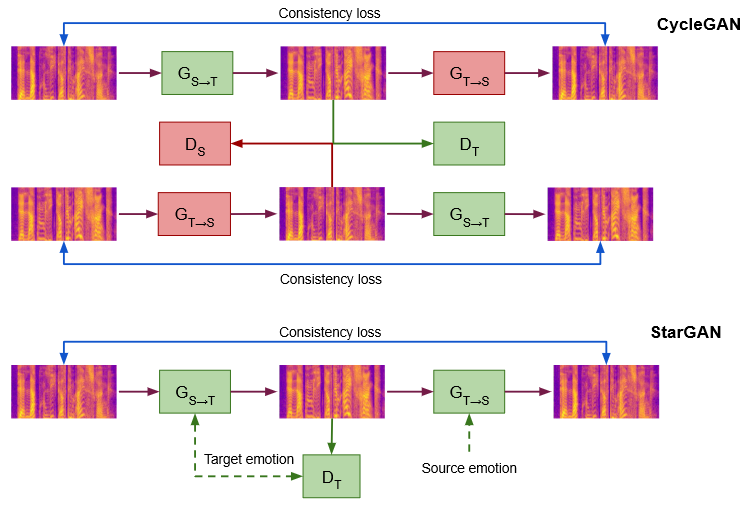
\includegraphics[width=0.4\textwidth]{"Bilder/GAN.PNG"}
\caption{The two most prevalent GAN approaches as depicted by \cite{triantafyllopoulos_overview_2023}}
\end{figure}

A common method for emotional speech synthesis on parallel data are so-called GANs \cite{goodfellow2020generative}. They consist of two neuronal networks, the generator and the discriminator. The generator is given a sentence with a specific emotion that it needs to transform into another emotion. After this task is done, the transformed sentence is given to the discriminator which also receives a naturally spoken sentence with the same emotion. The task of the discriminator is to distinguish between the naturally spoken and the generates sentence. In the learning process, generator and discriminator continuously improve themselves. Improvements of this method are the CycleGAN-VC \cite{kaneko2018cyclegan}, where two GANs translate between two different emotions such that the first GAN takes one emotion and transforms it into another emotion, and the second GAN takes this so generated emotion and transforms it back into the first emotion, and StarGAN-VC \cite{kameoka2018stargan} where generator and discriminator are trained to work on multiple domains.

In order to work on non-parallel data, the disentanglement method comes into use. The influences on the voice are thereby split into the content, the emotion and the speaker. Then different encoders are used to represent those influences.
Other demands of an affective speech synthesizer are that it controls the intensity of the emotion and that it allows a mixed emotion, for example a transition between sad and happy as it often happens in the mood swing of children. All in all, the synthesizers come to an accuracy of 50-80\% in studies. But their performance greatly depends on the environment, number and kind of emotions, language, culture, acceptance of user input and the resistance against noise \cite{triantafyllopoulos_overview_2023}.


\subsection{Competing Approaches}
\label{competing_approaches}
We will now take a look on some research in higher detail as to use it for the later evaluation. 

Our first comparison is to the Affect Editor of \cite{cahn_generation_2000}. As written in the previous section, Cahn's editor can be called the first real ETTS synthesizer. It encodes the emotion with the use of an acoustic model, where parameters encode important values like pitch, timing, voice quality and articulation. The inputs are an utterance and an emotion. After an initial acoustic analysis, the utterance is supplied with fitting pauses, hesitation and pitch to convey the emotion. \\
In comparison to Cahn's method, our simple approach uses a similar idea in terms of finding appropriate values to the most important acoustic features such as pitch, volume and timing. In contrast to the previously described method, the creation of the TTS audio is based on a state-of-the-art model and the transformation is simplified.\\
Our second comparison is to a novel approach by \cite{diatlova_emospeech_2023}. Based on the FastSpeech2 TTS architecture \cite{ren2020fastspeech}, they constructed their emotional TTS (EmoSpeech) model. FastSpeech2 is an encoder-decoder architecture which uses a feed-forward transformer block, a stack of multihead self-attention layers and 1D-convolution. With the use of embedding tables and FastSpeech2's eGeMAPS predictor, emotion is then projected on FastSpeech2's output on an utterance level. \\
In our first approach we used XTTS-v2, a TTS model developed by \cite{casanova2024xtts} from Coqui capable of synthesizing speech with controllable speaker identity. By providing the model model with a audio reference containing a emotional speaker characteristic, we were able to create an audio from a given text, which also contains the emotion of the speaker. \\
Instead of using a reference audio for emotion transfer, EmoSpeech utilizes explicit emotional embeddings that are trained on the emotion-labeled Emotional Speech Database (ESD) \cite{zhou2022emotional}. Unlike our first approach that uses XTTS-v2, which can generalize to new speakers and emotions dynamically, EmoSpeech is limited to the speakers and emotion categories present in its training data. Additionally, this allows XTTS-v2 to adopt new emotions with a short reference sample, while EmoSpeech requires further training on a dataset including this emotion.   

The reason for the choice of these two papers is that one of them is a deep dive into the history of ETTS and the other one is a modern method using current deep learning technology. Above all that, they use similar human-based evaluation techniques that can be combined and compared to our approaches.

\section{Methodology}
\label{methodology}
In this section, we will explain our methodology. The basis is a method described by \cite{bohra_smart_2022}. The input is a single textual sentence. In the first step, the prevalent emotion is extracted with the help of a large language model (LLM). Then the text is transformed into (neutral) speech. Now starts the actual emotion embedding and our own work which is diverging from Bohra's method.

While the two approaches we followed differ widely, we can still subdivide them further into a pre-processing, model application and post-processing phase. During the pre-processing, the audios are transformed into sequences or values, that are less dependent on the actual audio. Those are fed into the neural network together with the emotion. The output is the transformation that the audio needs to undergo in order to display the wished emotion. In the final step, this transformation is undertaken.

\begin{figure}[h]
 \centering
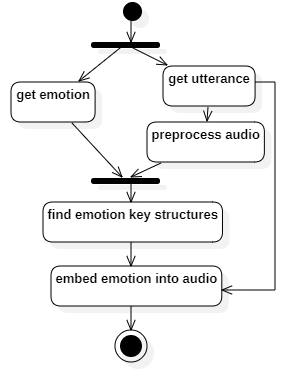
\includegraphics[width=0.4\textwidth]{"Bilder/Prozess.PNG"}
\caption{Depiction of the general method of our two approaches}
\label{Ablauf}
\end{figure}

\subsection{Training and Validation Data}
We used two separate datasets to train and validate different parts of our data.
The first one is the CERER \cite{saravia-etal-2018-carer} dataset. It contains 417 thousand sentences with annotated emotion labels. The annotated emotions are joy, sadness, fear, anger, love and surprise. We used it to validate the emotion recognition step of our procedure.

The second dataset is CREMA-D \cite{cao_data}, a dataset of 7,442 audio recordings taken by professional actors. It consists of twelve distinct sentences that are spoken by 91 different people and with different emotions, ranging over neutral, anger, disgust, fear, happiness, and sadness. The value of this dataset lies in that the neutral audio clip supplies us with some kind of ground truth as it is comparable to the utterances, our TTS step produces. Thus we can train a model on the comparison between neutral and emotional sentences of each speaker.

In order to use emotions that both datasets know, we create the intersection of the emotions: Joy (happiness), sadness, anger, and fear. Additionally, we add a neutral category.
\subsection{Text-To-Speech}
Text-to-speech (TTS) deals with the problem of converting normal language text into spoken words mostly in the form of an audio signal. 
In the current development environment, there are multiple advanced TTS libraries like Tacotron2 by \cite{shen_natural_2018} from NVIDIA, Google text-to-speech (gTTS) \cite{gtts} or Azure AI Speech\footnote{\url{https://azure.microsoft.com/en-us/products/ai-services/ai-speech/}} of Microsoft. For simplicity reasons, we decided to use gTTS for \hyperref[Experiment 1]{experiment 1} of \hyperref[approach 1]{approach 1} and for \hyperref[approach 2]{approach 2}. Initially gTTS used a concatenative and parametric speech synthesis. In later versions it utilized WaveNet, a deep generative model developed by \citeauthor{van2016wavenet} from DeepMind which is able to directly generate raw audio wave forms from given text. Another model worth mentioning is the XTTS-v2 \cite{casanova2024xtts} model from Coqui, which we will describe further in our \hyperref[Experiment 2]{Experiment 2} of \hyperref[approach 1]{approach 1}.

\subsection{Emotion Recognition}

The second ground stone of the information extraction is the emotion recognition. I used the Emotion English DistilRoBERTa-base\cite{hartmann2022emotionenglish}, which is trained to recognize six emotions: joy, sadness, anger, disgust, surprise and fear. The model performs well on the testing set in that it classifies 92\% of the emotions correctly. Only 19\% of the mismatched information are classified into the two emotion categories, that are not part of the input for our model. As for disgust we deal with it by classifying it as the most likely other known class, which is anger (87\%). Surprise is more differentiated, therefore it is evaluated further by enhancing the sentences with the allowed emotions and giving it to the model again. If the model recognizes another emotion, this one is preferred, otherwise the sentence is given a neutral co-notation. This improves the misinterpretation of surprise up to 73\%.

The whole procedure can be thus described as follows:
{
\small
\begin{equation*}
E(s)=\begin{cases}
  anger & \text{if } model(s)=disgust\\      
  max(model(emo_i+s)) & \text{if }  model(s)=surprise\\
  model(s) & \text{otherwise } 
\end{cases}
\end{equation*}
}
where $E$ is the emotion recognition algorithm, $s$ is the sentence model is the output of the Emotion English DistilRoBERTa-base, and $emo_i$ is a list of all allowed emotions integrated into the sentence "I am very *." in different variations.
This procedure pushes up the classification accuracy to 93\%.

\subsection{Approach 1 - Deep Learning Based}
\label{approach 1}
Our first approach is about using recent deep learning methods to generate an emotional audio. \\
Therefore we carried out two experiments:
\begin{enumerate}
	\item Training a transformer based model on prediction the emotional audio from a neutral one.
	\item Using the TTS model XTTS-v2 by \cite{casanova2024xtts} and its voice cloning ability to mimic not only the speaker but also its emotion.
\end{enumerate}

\subsubsection{Neutral-To-Emotional Transformer}
\label{Experiment 1}
Most state of the art TTS models like FastSpeech2 \cite{ren2020fastspeech} EmoSpeech \cite{diatlova_emospeech_2023} which is build upon FastSpeech2 rely on transformers alongside with attention. Therefore with our first experiment we tried to build a transformer based model for affective speech synthesis. The main idea is to train one model for each of the emotions: anger, sadness, happiness, fear and disgust. \\
The raw audio waves need to be pre-processed. First the audio waves from the previously mentioned emotion-labeled CREMA-D dataset \cite{cao_data} which contain full sentences for each sample are cropped into into smaller equal-length parts using a sliding window. This not only increases the total number of samples the model can train on, it also ensures they all have the same length. Second each audio crop is converted into one Mel scale spectrograms. It is created by applying the Short-Time Fourier Transform (STFT) to the an audio waveform and mapping the frequencies to the Mel scale using a filter bank. The result is a time-frequency representation where intensity indicates amplitude \cite{allen1977short}. \\
Our model consists of a transformer-encoder and -decoder. While training, it takes the Mel spectrogram of a neutral audio as input and the Mel spectrogram of the target emotion. It's important that the speaker and the crop position in the audio are equal for input and target. With a mean squared error (MSE) loss it compares the generated spectrogram with the target spectrogram and will later be used for backpropagation. \\
The neutral audio wave, which is used for generating the emotional audio is created with gTTS \cite{gtts}, a TTS model from Google. While inference the model segment-vise predicts the Mel spectrogram of the target emotion from a neutral one. The so predicted emotional Mel spectrogram needs to be converted back into one audio waveform. This is done by the Griffin-Lim Algorithm by \cite{griffin1984lim}, a phase reconstruction method based on the redundancy of the STFT. The gained audio waves should now represent the target emotion and text.

\subsubsection{Emotion Insertion using XTTS-v2}
\label{Experiment 2}
In our second experiment we use a more direct approach for generating emotional audio. To achieve this we used the XTTS-v2 model \cite{casanova2024xtts}, a TTS model which is capable of cloning the voice of a reference speaker. \\
The model consists of multiple components. A pre-trained GPT-2 transformer model \cite{radford2019language} at its core for predicting audio tokens from text tokens generated by a pre-trained Vector Quantised-Variational Autoencoder (VQ-VAE) \cite{betker2023better, NIPS2017_7a98af17}. A speaker and emotion conditioning module that extracts prosody, rhythm, pitch, and timbre features from the Mel spectrogram of a given reference audio. These extracted features guide the GPT-2 decoder in generating a Mel spectrogram that preserves the speaker characteristics of the reference. Finally the HiFi-GAN \cite{kong2020hifi} vocoder transforms the Mel spectrogram into a audio waveform. The so generated audio contains the given text sounding like the speaker from the reference audio. \\ 
We used this model to generate an emotional-sounding audio. To achieve this, the reference audio needs to contain the target emotion so the model can extract its characteristic. As source of our reference audio samples the emotion-labeled CREMA-D \cite{cao_data} dataset is used. From this dataset two speakers were selected, one female and one male. Important was that both speakers must have a clear recording of their voice with an expressive emotion. Dependent on the target emotion, a reference with one of the emotions anger, sadness, happiness, fear and disgust is selected from the dataset. Because the output audio of the XTTS-v2 model often contains background noise, a denoiser is applied. One negative side effect of denoising is that the volume is unevenly reduced. To rectify this, we segment-vise readjusted the volume of the audio before denoising, by comparing the peaks of each segment.

\subsection{Approach 2 - Acoustic Feature Based}
\label{approach 2}
The sound of our speech is deeply correlated with acoustic effects which themselves stem from the mouth movement and form\cite{arias_beyond_2020}. It is therefore evident that by manipulating the acoustic characteristics, an emotion can be conveyed.

The following transformations are implemented and can be applied to transform the audio:
Piecewise stretching, piecewise volume change, piecewise pitch change, emphasis/de-emphasis, pauses. The characteristics of acoustic, especially the logarithmic attributes of volume, are heeded whenever it doesn't impact the computation time and quality.
In total, the algorithm looks as can be seen in Algorithm \ref{alg:cap}.


\begin{algorithm}
\caption{write\_audio (audio, stretching\_list, volume\_list, pitch\_list, pause, emphasis)}\label{alg:cap}
\begin{algorithmic}
\State $audio \gets librosa.trim(audio)$
\If{$pause !=0$}
	\State $audio  \gets  add\_pause(audio,pause)$
\EndIf
\State $parts \gets segment(audio,len(stretching\_list))$
\For{$\textit{i,part in parts}$}
\State $temp  \gets  stretch(part, stretching\_list[i])$ 
\State $temp \gets volume (temp, volume[i-1], volume[i], emphasis)$
\State $temp \gets pitch (temp, pitch\_list[i])$
\State $parts[i] \gets temp$
\EndFor
\State $\gets combine(parts)$
\end{algorithmic}
\end{algorithm}


Sadness can be displayed by slowing down the whole audio and letting the volume and pitch drop down in the end of the sentence. Happiness in contrast can be included by increasing pitch and volume at the end. Finally, anger and fear can be symbolized by increasing the emphasis on each syllable. Fear also needs a distinct harmonic that we tried to apply via vibrations and noise, but that still needs improvement.


\subsection{Implementation}

In order to implement a usable synthesizer, I created a GUI application. It consists of a text input for the sentence. With the click on a checkbox, the sentence is evaluated in order to find the underlying emotion. If the checkbox is not selected, one can choose an arbitrary emotion instead. 

\begin{figure}[h]
 \centering
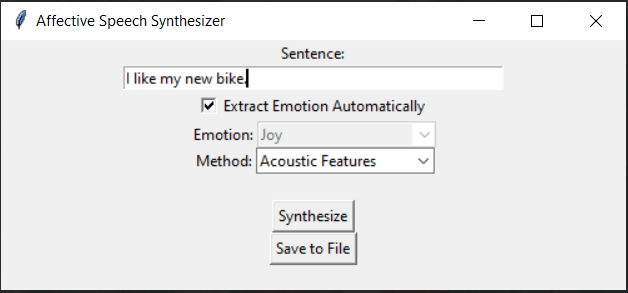
\includegraphics[width=0.4\textwidth]{"Bilder/gui_v2.png"}
\caption{GUI of the implementation}
\end{figure}

The sentence is then synthesized using the procedure in Figure \ref{Ablauf}. Therefore two methods are available select in the application which represent our two approach. The complication is here to choose suitable python libraries to create and transform the audio clip. Google text-to-speech \cite{gtts} saves its output in a designated gTTS class which has no options for transformation but can only be saved. In contrast, to get attributes like the volume or pitch of the audio or split it in segments, it needs to be transformed into another format. For simple transformations, it suffices to parse the audio into the AudioSegment format. Because the pitch is a complex attribute and not directly visible within the wave form of a audio, it needs more advanced functions, which can be found in the Librosa library \cite{McFee2015librosaAA}. The same is to be said for stretching an audio, since a simple time stretch would not only change the length of the audio but also its frequencies and therefore the pitch.
Finally, the audio clip is ready. It is replayed and can be saved to a file.

\section{Evaluation}
\label{evaluation}

\subsection{Benchmark}
One of the ongoing problems of ETTS is that there isn't a global benchmark yet\cite{triantafyllopoulos_overview_2023}. Every paper uses their own methodology and testing dataset. In contrast, we want to propose a benchmark. The benchmark is separated in to two datasets containing 12 sentences each. Some of them are taken from the CERER \cite{saravia-etal-2018-carer} dataset.

The first sentence collection contains simple sentences that don't have any subclauses. They are used to gather information about the general emotion representation in the spoken sentences. The second set of sentences contains sentences that have at least one subclause. The sentences are ordered by their length and should be used to prove that the algorithm can also work on non-standard sentences.

The sentences are then interlaced with the five emotions anger, happiness, sadness, fear and disgust. Additionally, there is a neutral category. One or more study participants listen to the sentences and annotate them with an emotion.


\subsection{Results}
\begin{table*}[t]

\centering
\vspace{5px}
{
\begin{tabular}{|p{2cm}|p{1.5cm}|p{1.5cm}|p{1.5cm}|p{1.5cm}|p{1.5cm}|p{1.5cm}|p{1.5cm}|}
\hline
\rowcolor{mintgreen}&neutral&anger&happiness&sadness&fear&surprise&disgust\\
\hline
\cellcolor{gainsboro}Approach 1&62.5&45.8&50.0&66.7&33.4&-&29.2\\
\hline
\cellcolor{gainsboro}Approach 2&87.5&45.8&50&62.5&12.5&-&-\\
\hline
\hline
\cellcolor{gainsboro}Affect Editor& -&65.5&83.2&97.1&72.7&72.7&80.7\\
\hline
\cellcolor{gainsboro}EmoSpeech&56 &94&80 &83&-&100&-\\
\hline
\end{tabular}
}

\caption{Comparison between the quantitative evaluations of the Affect Editor \cite{cahn_generation_2000}, EmoSpeech \cite{diatlova_emospeech_2023} and our approaches (in percent). Our approaches used the above described benchmark.}
\label{Tabelle2}
\end{table*}
In this section, we will use our benchmark to compare our approaches. We will also compare our outcomes to each other and to two approaches of other researchers, that were already described in Section \ref{competing_approaches}. You can refer to Table \ref{Tabelle2} for the full benchmark data and similar data of the compared papers.

The metric of the comparison is a problem in itself, as ETTS has no uniform evaluation method or a benchmark. A common method of evaluation is to let people listen to the audios and then sort them according to the emotion they mean to hear. This is the method that is also used in our two reference papers. But the type and complexity of the sentences used is not given and metrics like clarity are not considered, so the comparison is rudimentary. This can also be seen in that the Affect Editor \cite{cahn_generation_2000} and EmoSpeech \cite{diatlova_emospeech_2023} show comparable results despite their difference in up-to-dateness. Therefore, the evaluation has to be taken with a grain of salt.

The algorithms can have two sources of error. The first one lies in the emotion recognition. Based on the CARER dataset \cite{saravia-etal-2018-carer} we can say, that the accuracy of this part lies at 93\%. The second risk of failure lies in the embedding of the emotion into the audio. Here our two approaches differ.

\begin{table}[h]

\small
\vspace{5px}
{
\begin{tabular}{|p{0.9cm}|p{0.65cm}|p{0.65cm}|p{0.65cm}|p{0.65cm}|p{0.65cm}|p{0.65cm}|}
\hline
\rowcolor{mintgreen}&neutral&anger&happy&sad&fear&disgust\\
\hline
\cellcolor{gainsboro}easy&66.7&33.3&50.0&41.7&50.0&41.7\\
\hline
\cellcolor{gainsboro}advanced&58.3&58.3&50.0&91.7&16.7&16.7\\
\hline
\end{tabular}
}

\caption{Comparison of the simple and advanced benchmark sentences for \hyperref[approach 1]{approach 1} (in percent).}
\label{Tabelle3}
\end{table}
When comparing the results of \hyperref[approach 1]{approach 1} on the easy and advanced benchmark sentences as seen in Table \ref{Tabelle3} it can be shown that happiness and sadness can be separated well, while disgust and fear are hard to not good represented. This might be because the  emotional expression for happy and sad are much stronger than for fear and disgust or anger. Another possible reason could be that while evaluation it is hard for a human listener to distinguish between e.g. anger and disgust. Also the approach works better with longer or more advances sentences. \\   
For the used evaluation metric, \hyperref[approach 1]{approach 1} is worse than EmoSpeech \cite{diatlova_emospeech_2023} in every emotion category except neutral, where it is slightly better (see Table \ref{Tabelle2}). It is worth mentioning that EmoSpeech uses less in number but more distinctive emotions than our approach, which makes it easier to distinguish the individual ones. 

\begin{table}[h]

\small
\vspace{5px}
{
\begin{tabular}{|l|l|l|l|l|l|}
\hline
\rowcolor{mintgreen}&neutral&angry&happy&sad&fearsome\\
\hline
\cellcolor{gainsboro}easy&83.3&58.3&58.3&53.3&25\\
\hline
\cellcolor{gainsboro}advanced&91.7&33.3&41.7&66.6&0\\
\hline
\end{tabular}
}

\caption{Comparison of the simple and advanced benchmark sentences for \hyperref[approach 2]{approach 2} (in percent).}
\label{Tabelle4}
\end{table}

\hyperref[approach 2]{Approach 2} performs well in the quantitative analysis of Table \ref{Tabelle2}, but not as good as \cite{cahn_generation_2000} on any of the comparable emotions. It also has the same qualitative problems that might compromise the Affect Editor. The emotion, while clearly embedded, tends to be comically emphasized, especially in the case of sadness. It's also visible that fear is not displayed as well as other emotions. Neutral emotions on the other hand, are directly transported from the TTS and therefore well represented.

The approach scales surprisingly well for complex sentences that contain subclauses, as seen in Table \ref{Tabelle4}, even outperforming the easy benchmark in two of the categories. The same is not to be said for the quality of the emotional display, which gets even more distorted.

If set into relation, one can say that our approaches generally perform less well than those described in the two scientific papers. Nonetheless, the tendencies are similar. Both approaches have strengths and weaknesses in different areas but are comparable in the mean precision, which is 47.9 \% for \hyperref[approach 1]{approach 1} and 51.7 \% for \hyperref[approach 2]{approach 2}.

\section{Discussion}
\label{discussion}
Let's first discuss our outcomes.
Even though the model's architecture is similar to models like FastSpeech2 \cite{ren2020fastspeech}, the results from the \hyperref[Experiment 1]{first model} of \hyperref[approach 1]{approach 1} where not so promising. This is why we decided to exclude them from evaluation and focus on the \hyperref[Experiment 2]{second experiment}. \\
We compared two transformer based approaches, the \hyperref[Experiment 2]{second experiment} of \hyperref[approach 1]{approach 1} against the EmoSpeech model \cite{diatlova_emospeech_2023}. By comparing just the raw benchmark scores, EmoSpeech performs way better than our approach of using XTTS-v2 \cite{casanova2024xtts} with an additional emotional audio as reference. Besides this performance difference, our approach has a advantage. While EmoSpeech can only handle emotions that occurred in the training dataset, which limits the number of possible emotions that can be represented by the model, our approach can adopt on the nearly every emotion of the reference audio. That also makes XTTS-v2 and so our approach more flexible since it does not need to be trained again on a new emotion. \\
Over all both models have its benefits, but when it comes to generating a audio with an emotion of a fixed set of emotions the EmoSpeech model performs best.

As for \hyperref[approach 2]{approach 2}, we could see in the evaluation that fear is not displayed correctly, as its harmonies could not be modeled by the chosen parameters. In contrast, the neutral emotion category has improved in comparison to the Affect Editor both for easy and complex sentences, which can be attributed to the improvement of general TTS. Another interesting fact is that when performing the transformations on naturally spoken sentences and generated sentences, the parameters had to be tuned differently. The spoken language had an even higher tendency to perform well with happiness and sadness, while anger wasn't displayed as well. The comparison can be seen in Figure \ref{fig:fig}. One can conclude that \cite{cahn_generation_2000} had to tune his Affect Editor differently than our approach.

In general, our acoustics approach is less good than the Affect Editor, as it is programmed in a shorter time and less flexible. Changes that would influence the algorithm to the better is to vary the number and length of the chunks. This could be done by use of the Librosa split function or a mapping of words to the audio. Additionally, a shivering sound is needed for the fear emotion. Finally, the transformation should be adapted to the length of the sentence and ideally consider subclauses.


\begin{figure}
\begin{subfigure}{.5\textwidth}
\begin{subfigure}{.18\textwidth}
  \centering
  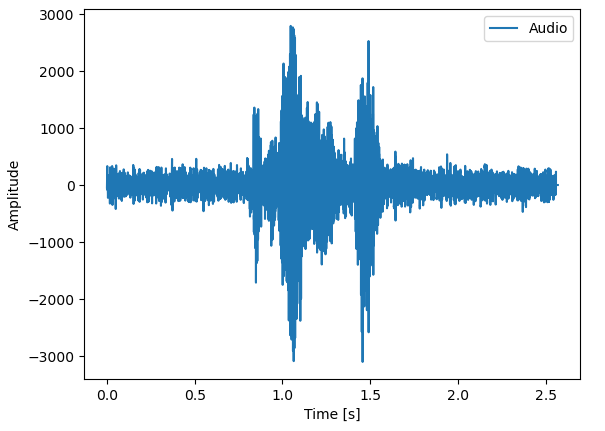
\includegraphics[width=\linewidth]{"Bilder/seminat_neutral.png"}
  \label{fig:sfig1}
\end{subfigure}%
\begin{subfigure}{.18\textwidth}
  \centering
  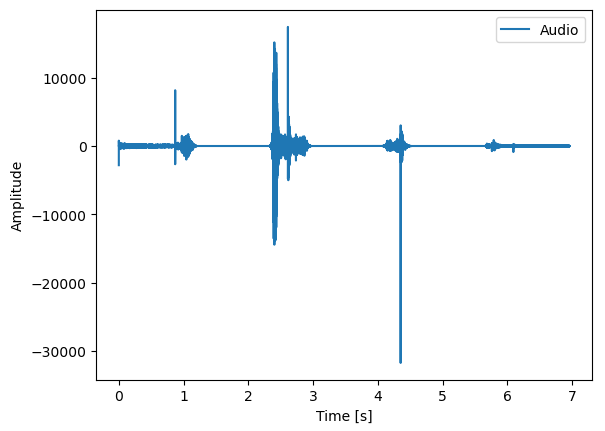
\includegraphics[width=\linewidth]{Bilder/seminat_angry.png}
  \label{fig:sfig2}
\end{subfigure}
\begin{subfigure}{.18\textwidth}
  \centering
  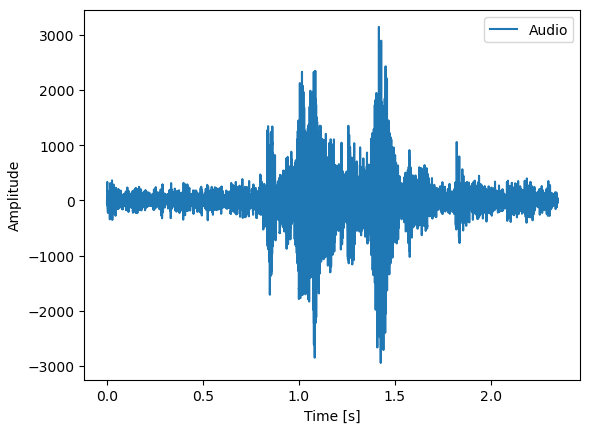
\includegraphics[width=\linewidth]{Bilder/seminat_happy.png}
  \label{fig:sfig2}
\end{subfigure}
\begin{subfigure}{.18\textwidth}
  \centering
  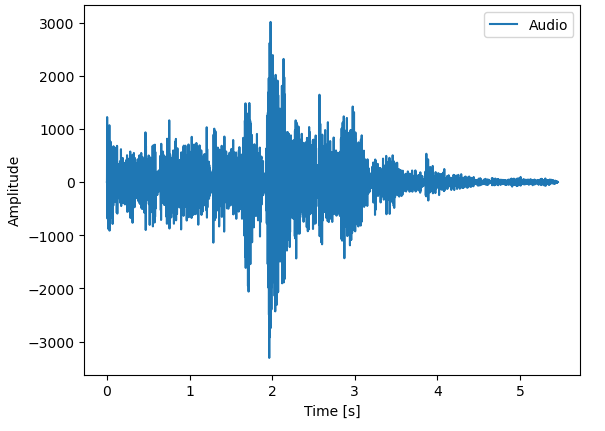
\includegraphics[width=\linewidth]{Bilder/seminat_sad.png}
  \label{fig:sfig2}
\end{subfigure}
\begin{subfigure}{.18\textwidth}
  \centering
  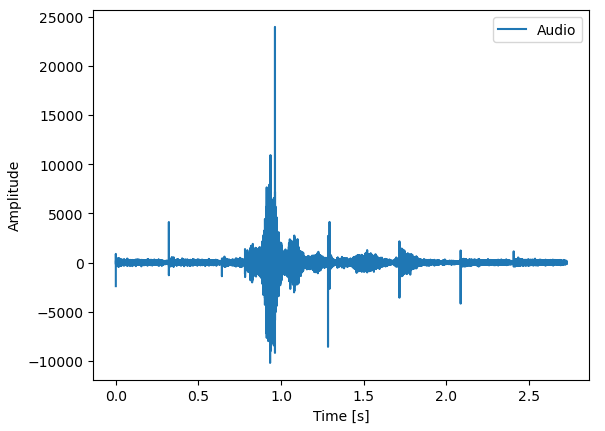
\includegraphics[width=\linewidth]{Bilder/seminat_fear.png}
  \label{fig:sfig2}
\end{subfigure}
\caption{Transformation on natural utterance}
\end{subfigure}

\begin{subfigure}{.5\textwidth}
\begin{subfigure}{.18\textwidth}
  \centering
  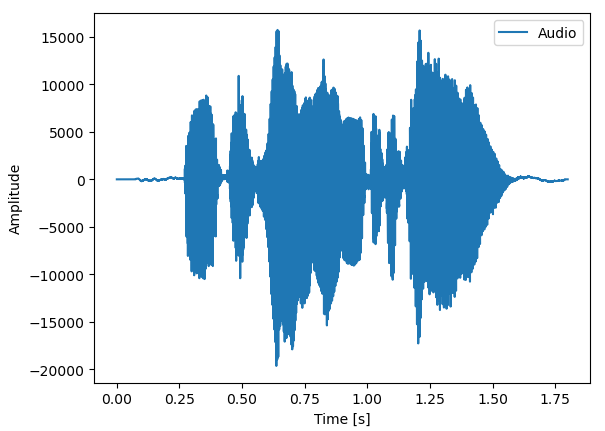
\includegraphics[width=\linewidth]{"Bilder/art_neutral.png"}
  \label{fig:sfig1}
\end{subfigure}%
\begin{subfigure}{.18\textwidth}
  \centering
  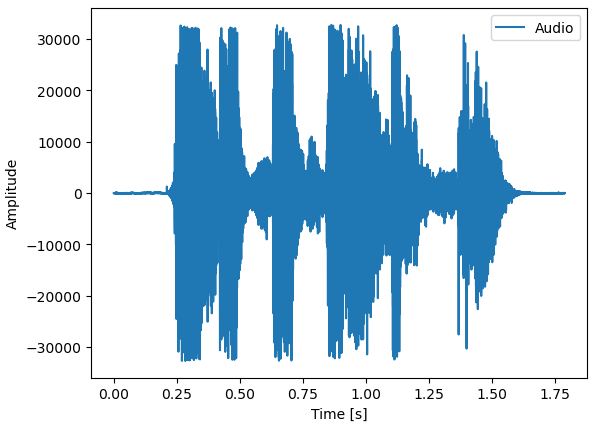
\includegraphics[width=\linewidth]{Bilder/art_angry.png}
  \label{fig:sfig2}
\end{subfigure}
\begin{subfigure}{.18\textwidth}
  \centering
  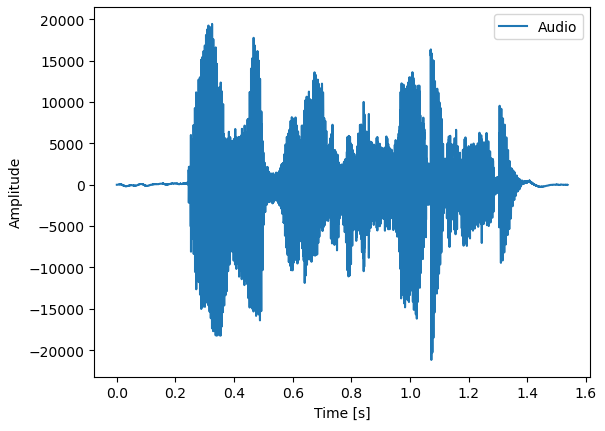
\includegraphics[width=\linewidth]{Bilder/art_happy.png}
  \label{fig:sfig2}
\end{subfigure}
\begin{subfigure}{.18\textwidth}
  \centering
  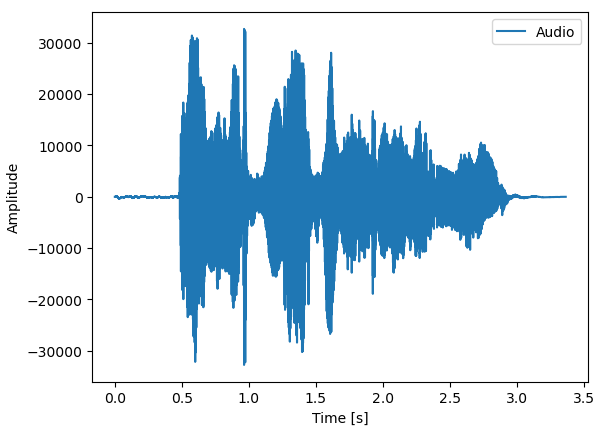
\includegraphics[width=\linewidth]{Bilder/art_sad.png}
  \label{fig:sfig2}
\end{subfigure}
\begin{subfigure}{.18\textwidth}
  \centering
  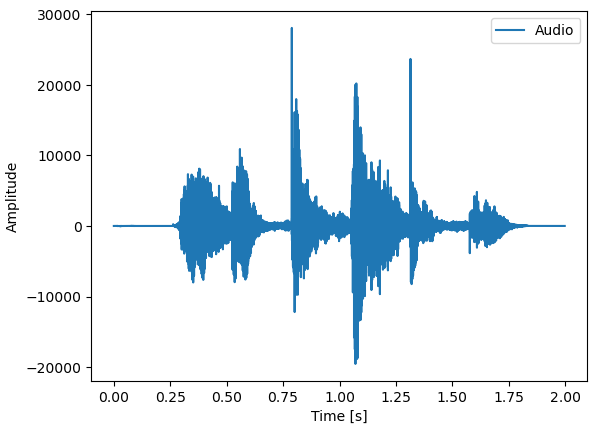
\includegraphics[width=\linewidth]{Bilder/art_fear.png}
  \label{fig:sfig2}
\end{subfigure}
\caption{Transformation on artificial utterance}
\end{subfigure}
\caption{Neutral audio and the created emotional audios (left to right): neutral, angry, happy, sad, fearsome}
\label{fig:fig}
\end{figure}
While our benchmark provides a strong improvement on comparability in the ETTS area, it also has a disadvantage. The procedure of the study is not written out in high precision. This is a voluntary decision, because a extensive study is out of the scope of this project, but if it is applied to a more advanced research setting, it should be extended with a concrete study setting. Because we did the evaluation ourselves instead of conducting a complete study, the evaluation might contain biases since we already knew the intrinsics of the algorithms.

Another important question is the general ethicality of improving the human-likeliness of synthesized speech. On the one hand, it improves the quality of generated speech. This could be very beneficial for both barrier improvement for blind people as well as translations, commercials, and artists (for example the dubbing of indie computer games). On the other hand, it allows for more believable deep fakes. It also poses the ever-present question of which data can be used for deep learning training without violating copyright. In our case, the data was taken from an open training set, but the given sets are sparse and as in our case too small to get optimal results\cite{he_improve_2022}. The risk of taking the needed training data from sources of questionable copyright such as audio books and quality such as noisy videos.

\section{Conclusion}
\label{conclusion}
It wasn't to be expected that a simple course project can hold up to the current highs scientific research. Yet we could find similar trends in our experiments as in the respective fields of science, unifying them in a single benchmark.

But our approaches and benchmark are restricted to single sentence with a single emotion albeit XTTS-v2 takes a step in the right direction of allowing arbitrary emotions.
As ETTS is constantly improving together with the advances in TTS, a more wholesome approach has to be taken eventually, where emotions are added with more subtlety and a mixture. This is the major direction where ETTS needs to go.

\section{Contribution Statement}
Hannes Bachmann: Text-to-speech, \hyperref[approach 1]{Approach 1} (main approach), benchmark

Julia Rennert: Emotion recognition, \hyperref[approach 2]{Approach 2}, find datasets, write "related work", benchmark

\section{Link to the Repository}
{\small\url{https://github.com/Iphled/Affective\_Speech\_Synthesis}}

Please note that the data is not in the repository as the audio files are too big. To test out the algorithms that require the audios, please download them from the dataset source described above, and add them to the project in a "data" folder.

% Create a file `references.bib'
% 
% @article{dijkstra1968goto,
%   title={Go To Statement Considered Harmful (1968)},
%   inproceedings={CACM},
%   author={Dijkstra, Edsger},
%   year={2021}
% }

%\bibliographystyle{acl}
\bibliography{NLP}


\end{document}
